\begin{tikzpicture}[line width = 1.2pt, scale = 2, line join=round,x=1cm,y=1cm,>=stealth]
	% Koordinatensystem
	\draw [->] (0,0) -- (3.6,0) node[anchor=north west] {$z$};
	\draw [->] (0,0) -- (0,1.5) node[anchor=east] {$ \geschw $};
	% Plot
	\foreach \e in {1,2,3} {\draw ({\e-1},0) -- ({\e},{1});
		\draw [dashed] ({\e},1) -- ({\e},0);}
	\draw (3,0) -- (3.5,0.5);
	\draw (1,0) node[anchor = north] {$\tau$};
	\draw (2,0) node[anchor = north] {$2 \tau$};
	\draw (3,0) node[anchor = north] {$3 \tau$};
	\draw [dashed] (3.5,1) -- (0,1) node [anchor=east] {$ \dfrac{\partladung}{\masse} \cdot \efeld \cdot \tau $};
\end{tikzpicture}